\section{Convolutional Neural Networks}

  Convolutional networks work with images, so let's introduce a nice way to represent them as vectors. 

  \begin{definition}[Image]
    An image is a vector in some tensor product space. More specifically, avoiding the technicality that each pixel element is bounded and discrete,  

    \begin{enumerate}
      \item A grayscale image of resolution of $H \times W$ is a vector in $\mathbb{R}^{H} \otimes \mathbb{R}^{W}$. 

      \item An image with $C$ channels of the same resolution is an element of $\mathbb{R}^{C} \otimes \mathbb{R}^H \otimes \mathbb{R}^W$. 

      \item A video with $C$ channels and of the same resolution is an element of $\mathbb{R}^T \otimes \mathbb{R}^C \otimes \mathbb{R}^H \otimes \mathbb{R}^W$, where $T$ is the time dimension which is usually represented in some discrete frames.
    \end{enumerate}

    Since tensor product spaces are also vector space, there is nothing new we have to introduce. Everything we talked about so far applies to images when treated as vectors. In fact, so far we have been interpreting images of size $(C, H, W)$ through the isomorphism 
    \begin{equation}
      \phi: \mathbb{R}^{C} \otimes \mathbb{R}^H \otimes \mathbb{R}^W \rightarrow \mathbb{R}^{C \times H \times W}
    \end{equation}
    that essentially ``unravels" the image. 
  \end{definition}

\subsection{Convolutional and Pooling Layers} 

  So far, we have seen the power of multilayer perceptrons and their predictive ability on moderately sized vectors. In fact, if we process the MNIST with a simple MLP of 2 layers and 512 nodes each, we can easily get $95\%$ accuracy within 10 epochs. However, these MNIST pictures are extremely low resolution, at $1 \times 28 \times 28$, and for even moderately sized images we can that there is a huge blowup of parameters needed. \footnote{For example, an RGB image that is $3 \times 1024 \times 1024$ would have ~3m parameters, and then defining a dense linear map to even 1000 dimensions would take 3 billion parameters. Given that 32-bit floating point is $4$ bytes, this already takes up 12GB of memory just to load the network.} Clearly, this is not efficient, and so the only way to move on is to create a sparser representation of the network. This is where convolutional kernels come in (note that this is completely different than the kernels mentioned in supervised learning, with support vector machines and RKHS), introduced in \cite{cnn}. The general idea is to take a small dot product.

  \begin{figure}[H]
    \centering 
    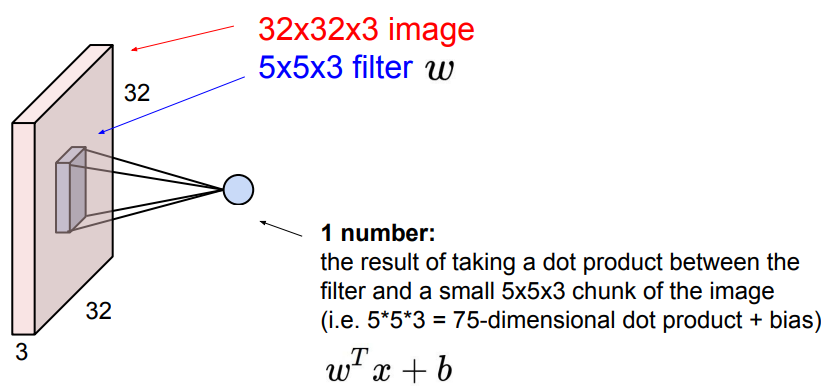
\includegraphics[scale=0.35]{img/kernel1.png}
    \caption{} 
    \label{fig:kernel1}
  \end{figure}

  \begin{figure}[H]
    \centering 
    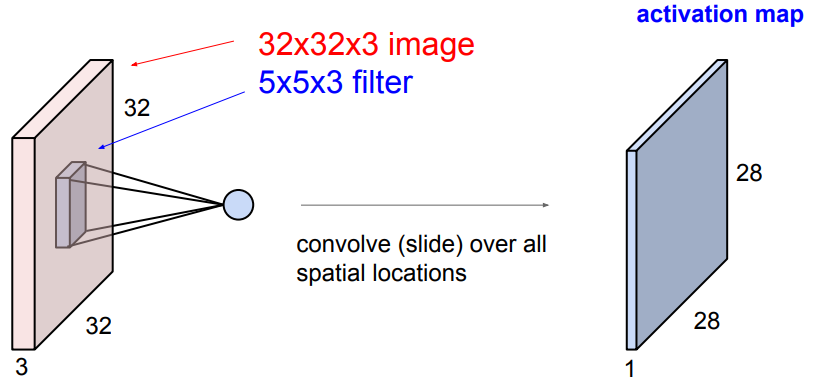
\includegraphics[scale=0.35]{img/kernel2.png}
    \caption{} 
    \label{fig:kernel2}
  \end{figure}

  \begin{figure}[H]
    \centering 
    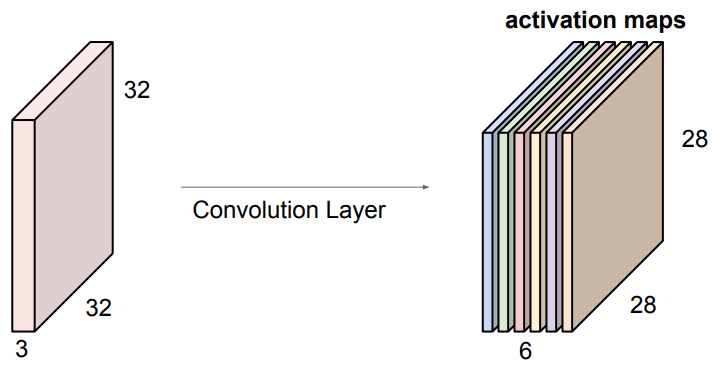
\includegraphics[scale=0.35]{img/kernel3.png}
    \caption{} 
    \label{fig:kernel3}
  \end{figure}

  \begin{definition}[Convolutional Kernel]
    A \textbf{convolution operator} on a vector space $V$ representing an image space is simply a special type of linear map that is parameterized by a much smaller set of numbers, stored within a \textbf{kernel} or \textbf{filter}. In all honesty, it is much easier to go through examples to see how they work, so in this definition I will focus more on describing the hyperparameters. Given an image of shape $(C, H, W)$, the convolution is essentially a sliding window that computes a dot product between the kernel and the window that the kernel covers over the image. 
    \begin{enumerate}
      \item The sliding window size is $(W_{ker}, H_{ker})$, which is conventionally square but does not need to be. 

      \item This sliding window must compute over all channels, so in fact it is of shape $(C_{in}, W_{ker}, H_{ker})$. This would generate one output channel image. 

      \item Multiple kernels can be used concurrently to generate different channel images. Therefore, if we want to have a collection of $C_{\text{out}}$ outputs that are extracted from each kernel, our total kernel would be a collection of $C_{out}$ kernels of shape $(C_{in}, W_{ker}, H_{ker}, C_{out})$. Therefore, the total equation is 
      \begin{equation}
        (X \ast K)_{f, i, j} \coloneqq \sum_c \sum_{p, q} X_{c, i + p, j + q} \cdot K_{c, p, q, f} + b_{f, i, j}
      \end{equation}

      where $c$ is the channel index, $p, q$ are the location indices, $f$ is the output channel index, and $b$ is some bias term. 

      \item The stride parameter $s$ can also be set to determine the stride of the kernel $\mathcal{K}$. 

      \item Another thing to note is that the output image of a kernel would be slightly smaller than the input image, since the kernel cannot go over the edge. However, there are padding schemes to preserve the original dimensions. 
    \end{enumerate}
    From the equation above, we can see that a convolutional layer, assuming that it has full padding, is a linear map  
    \begin{equation}
      \mathcal{K} : \mathbb{R}^{C_{in}} \otimes \mathbb{R}^H \otimes \mathbb{R}^W \rightarrow \mathbb{R}^{C_{out}} \otimes \mathbb{R}^H \otimes \mathbb{R}^W
      \label{eq:conv_mapping}
    \end{equation}
    The vector space of linear maps mapping between these two spaces has $C_{in} H^2 W^2 C_{out}$ dimensions, which is extremely large, but parameterizing $\mathcal{K}$ with this matrix reduces the set of relevant convolutional maps to a subspace that is $(1 + C_{in} H_{ker} W_{ker}) C_{out}$ dimensional (with the $+1$ due to a bias term, making this an affine map). This is essentially what a convolution is: sparse matrix multiplication, and there is nothing else that makes it different from a classical feedforward neural network. It's just computationally efficient matrix multiplication for high-dimensional vectors. 
  \end{definition}

  In addition to computational efficiency and weight sharing, convolutional operators capitalize on the principle of \textbf{locality}, i.e. that pixels are directly related to adjacent pixels. For example, a pixel representing a portion of a dog's ear would not be related to the background, but the color and positioning should be related to the dog's face, which may be within a certain neighborhood around. This has been shown to be similar to the human visual system and is thus well motivated. 

  Though this next topic has more to do with classical image processing than computer vision, there are a surprising number of features that these convolutional filters can extract from an image. By treating them as a discretized form of a partial derivative (as the vertical and horizontal edge detection) or as the Hessian operator (sharpening), we can extract many features from them.  

  \begin{example}[Blurs, Edge Detection]
    Given the original image below, we show various convolutional filters applied on the image. Note that the kernel matrix may have the property that all of its entries sum to $1$, meaning that on average, the expected value of the brightness of each pixel will be $0$, and the values will be left unchanged on average. However, this is not a requirement.  
    \begin{align*}
      \mathrm{Original} = \begin{bmatrix} 1 & 0 & 0 & 0 & 0 \\ 0 & 1 & 0 & 0 & 0 \\ 0 & 0 & 1 & 0 & 0 \\ 0 & 0 & 0 & 1 & 0 \\ 0 & 0 & 0 & 0 & 1 \end{bmatrix} & 
      \mathrm{Mean} = \frac{1}{25} \begin{bmatrix} 1 & 1 & 1 & 1 & 1 \\ 1 & 1 & 1 & 1 & 1 \\ 1 & 1 & 1 & 1 & 1 \\ 1 & 1 & 1 & 1 & 1 \\ 1 & 1 & 1 & 1 & 1 \end{bmatrix} & 
      \mathrm{Gaussian} = \frac{1}{273} \begin{bmatrix} 1 & 4 & 7 & 4 & 1 \\ 4 & 16 & 26 & 16 & 4 \\ 7 & 26 & 41 & 26 & 7 \\ 4 & 16 & 26 & 16 & 4 \\ 1 & 4 & 7 & 4 & 1 \end{bmatrix} \\   
      \mathrm{Sharpen} = \begin{bmatrix} 0 & -1 & 0 \\ -1 & 5 & -1 \\ 0 & -1 & 0 \end{bmatrix} & 
      \mathrm{Horizontal} = \begin{bmatrix} -1 & 0 & 1 \\ -2 & 0 & 2 \\ -1 & 0 & 1 \end{bmatrix} & 
      \mathrm{Vertical} = \begin{bmatrix} -1 & -2 & -1 \\ 0 & 0 & 0 \\ 1 & 2 & 1 \end{bmatrix} 
    \end{align*}

    These filters visually output the following images. Note that these filters are each acting on the image by acting individually on each channel and then combining the 3 outputs to create the new RGB image. 
    \begin{figure}[H]
      \centering
      \begin{subfigure}[b]{0.32\textwidth}
      \centering
          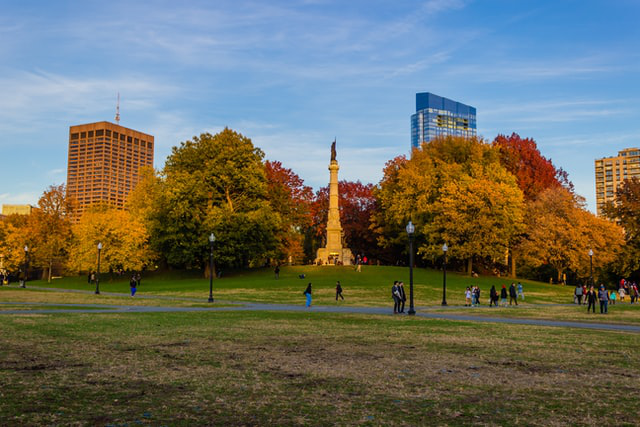
\includegraphics[width=\textwidth]{img/Park_Full.png}
          \caption{Original image. }
          \label{fig:original_image}
      \end{subfigure}
      \begin{subfigure}[b]{0.32\textwidth}
      \centering
          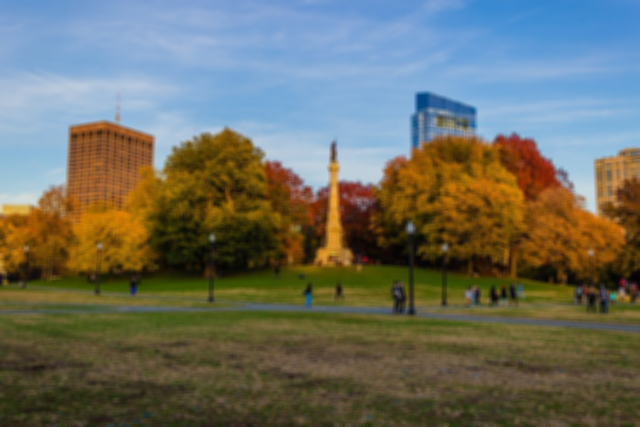
\includegraphics[width=\textwidth]{img/Mean_Blur.png}
          \caption{$5 \times 5$ mean blur applied. }
          \label{fig:mean_blur_image}
      \end{subfigure}
      \begin{subfigure}[b]{0.32\textwidth}
      \centering
          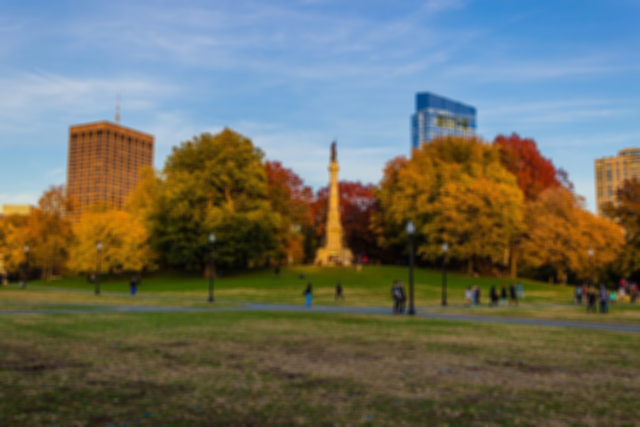
\includegraphics[width=\textwidth]{img/Gaussian_Blur.png}
          \caption{$5 \times 5$ Gaussian blur applied. }
          \label{fig:normal_blur_image}
      \end{subfigure}
      
      \begin{subfigure}[b]{0.32\textwidth}
      \centering
          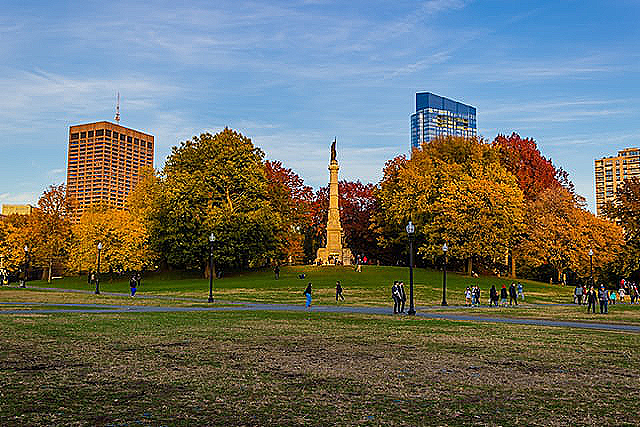
\includegraphics[width=\textwidth]{img/Sharpen.png}
          \caption{Sharpening kernel. } \label{fig:sharpened_image}
      \end{subfigure} 
      \begin{subfigure}[b]{0.32\textwidth}
      \centering
          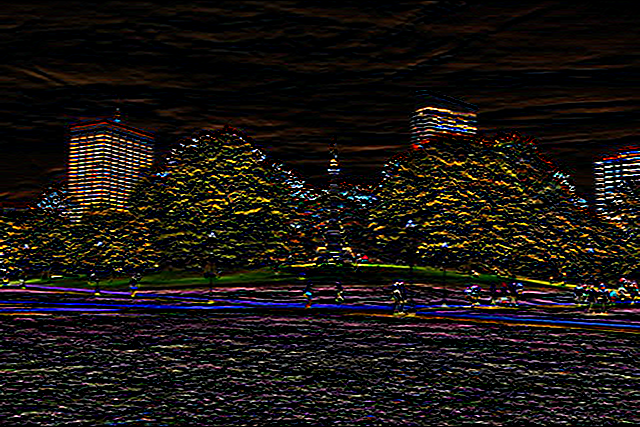
\includegraphics[width=\textwidth]{img/Horizontal.png}
          \caption{Horizontal edge detection. }
          \label{fig:horizontal_edge}
      \end{subfigure}
      \begin{subfigure}[b]{0.32\textwidth}
      \centering
          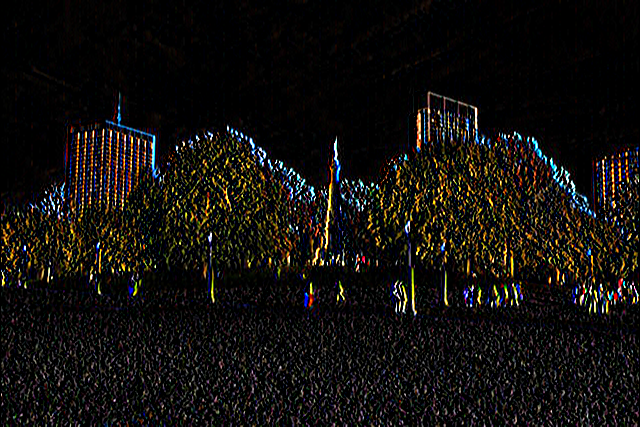
\includegraphics[width=\textwidth]{img/Vertical.png}
          \caption{Vertial edge detection. }
          \label{fig:vertical_edge}
      \end{subfigure} 

      \caption{Different convolutional kernels acting on the same image. Several useful features like edges can be detected with these simple linear maps. }
      \label{fig:feature_extraction}
    \end{figure}
  \end{example}

  We have seen in the example above that we can interpret each output channel of a convolution as a feature. That is, our original input image with $C_{in} = 3$ channels may go through a convolution that has $C_{out} = 10$ output channels, producing $10$ grayscale images. Each of these images may represent a feature that is extracted from the image through a custom kernel. When we stack convolutional layers together (with nonlinearities in between, of course), we can produce more complicated transformations that extract more abstract features. For example, while the first layer or two may extract certain edges within a dog, perhaps the fourth or fifth convolutional layer will be able to detect the presence of ears. This is a hand-wavy example, but if you actually visualize the outputs of these layers during forward prop, it is possible to see this in action.  

  What we eventually hope for is that we can extract higher level features that can be encoded in moderate-dimensional vectors. Unfortunately, the rate at which regular convolutional filters (especially when there is padding and a stride of $1$) does not shrink the resolution of the input images at a fast enough rate. For example, having a $3 \times 3 \times 3 \times 3$ kernel with no padding on a $(3, 100, 100)$ image will decrease the dimensions to only $(3, 98, 98)$ only. Therefore, we do some very simple operations to reduce the resolution faster. 

  \begin{figure}[H]
    \centering 
    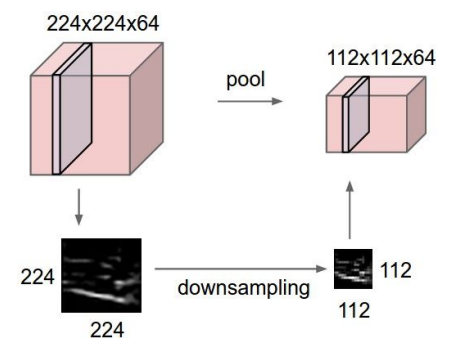
\includegraphics[scale=0.4]{img/max_pool1.png}
    \caption{} 
    \label{fig:max_pool1}
  \end{figure}

  \begin{figure}[H]
    \centering 
    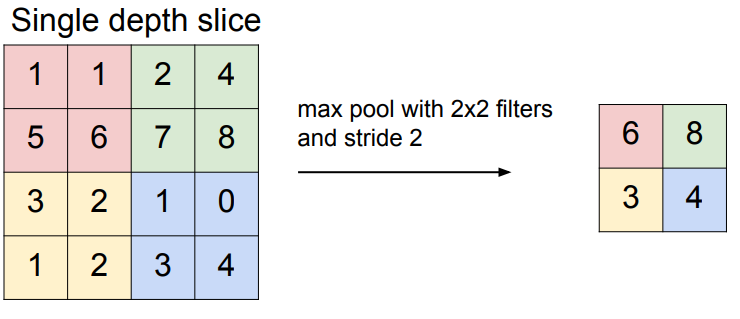
\includegraphics[scale=0.4]{img/max_pool2.png}
    \caption{} 
    \label{fig:max_pool2}
  \end{figure}

  \begin{definition}[Pooling Layers]
    A pooling layer takes in an input image of dimension $(C, H, W)$ and essentially does \textbf{downsampling} on it, involving some method of pooling local groups of pixels together into one value. There are several ways to do this: 
    \begin{enumerate}
      \item \textbf{Max Pooling} refers to dividing each channel of the image into a ``checkerboard" of $P \times P$ (where $P$ is a hyperparameter and does not necessarily have to be a square) matrices and simply choosing the maximum pixel value from it. 
      \item \textbf{Average Pooling} is the same as max pooling but we just take the average. 
    \end{enumerate}
    Clearly, these are not expensive operations and are an effective way to downsample. Therefore, the same $(3, 100, 100)$ image, after one convolutional layer followed by a pooling layer, will result in a $(3, 49, 49)$ image.  
  \end{definition}

  Ultimately, after a series of convolutions and pooling, we would want to reduce this image to a form of $(C, H, W)$, where both $H$ and $W$ are small and $C$ is large. This is because for each value of $C$, say $C = 1$, the cross section $\{(1, W, H)\}$ would encode the value of the feature identified by $C$. In fact, it could be the fact that both $H$ and $W$ are $1$, and $C = 10$. Then, we would essentially be looking at an array of $10$ numbers, which could encode the presence of some abstract features. For example, the first value $C = 1$ would encode the presence of an eye, which in the end has a value of $0.9$ (high probability), the second $C = 2$ could encode the presence of an ear, and so on. 

  Perhaps the sparsity of these maps may not allow the convolutional layers alone to extract all the features we need, so it is common to unwrap the features and then add a few fully connected layers at the end, which is much more computationally feasible now that the convolutions and pooling layers have reduced the dimensionality whilst extracting useful features with the concept of locality. This turns out to have comparable performance to regular MLPs with a fraction of the computational cost, and can easily reach $98\%$ validation accuracy on the MNIST dataset. 

  \begin{center}
    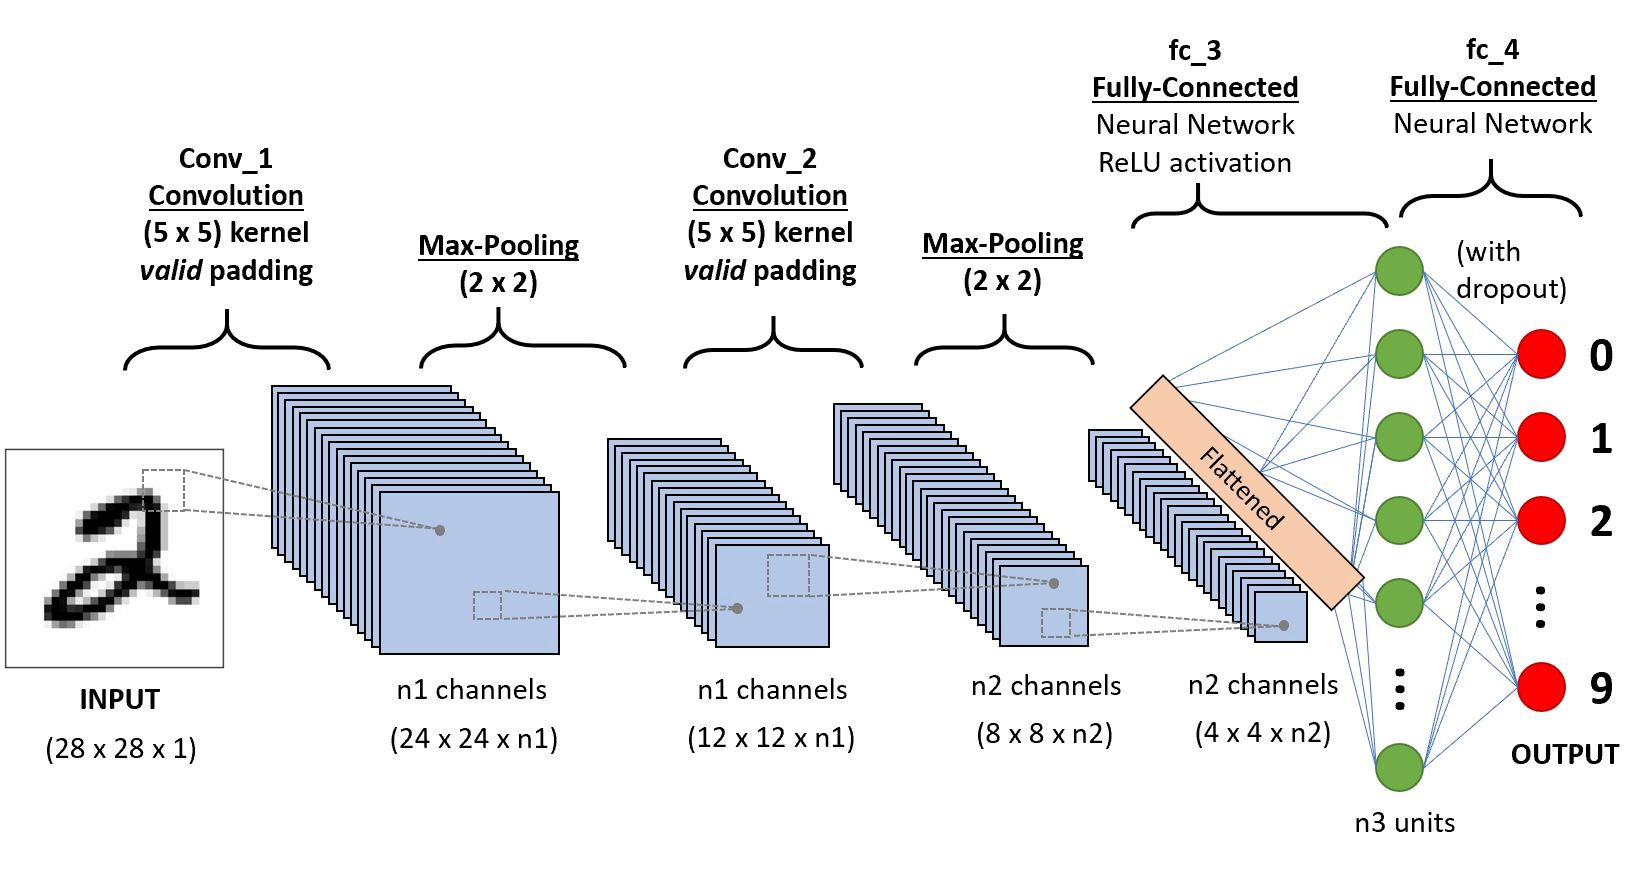
\includegraphics[scale=0.25]{img/CNN_architecture.jpeg}
  \end{center}

\subsection{Backpropagation}

  The fully connected layers are all taken care of, but now it's the convolutional layers and the pooling layers. The convolutional layers are also linear maps, so they can be treated the same way. However, the pooling layers may be nonlinear. 
  \begin{enumerate}
    \item Average pooling is linear, so no worries here. 
    \item Max pooling is not linear, but it is the next best thing: piecewise linear. 
  \end{enumerate}

\subsection{Visualizing Activation Maps}

  \subsection{CAM and Grad-CAM}


\subsection{Exercises}

  \begin{example}[Tarokh, Duke ECE685]
    Consider an RGB image $X = [X_0, X_1, X_2]$ with three channels, and given as follows 

    \begin{equation}
      X_0 = \begin{bmatrix} 2 & 1 & 0 & 0 \\ 0 & 0 & 2 & 1 \\ 0 & 2 & 0 & 1 \\ 2 & 1 & 0 & 1 \end{bmatrix}, \;\; 
      X_1 = \begin{bmatrix} 2 & 2 & 0 & 0 \\ 0 & 0 & 2 & 1 \\ 0 & 0 & 2 & 0 \\ 0 & 1 & 0 & 1 \end{bmatrix}, \;\; 
      X_2 = \begin{bmatrix} 2 & 1 & 0 & 0 \\ 0 & 0 & 2 & 1 \\ 2 & 0 & 0 & 0 \\ 0 & 1 & 0 & 1 \end{bmatrix}
      \label{eq:tarokh_conv_exercise}
    \end{equation}
    
    The image is passed through the convolutional filter with the weights $W = [W_0, W_1, W_2] \in \mathbb{R}^{3 \times 3 \times 3}$ and step size $1$, and given as follows 

    \begin{equation}
      W_0 = \begin{bmatrix} 1 & 0 & 0 \\ 0 & -2 & 0 \\ 0 & 0 & -1 \end{bmatrix}, \;\; 
      W_1 = \begin{bmatrix} 1 & 2 & 0 \\ 2 & 0 & - 1 \\ 0 & -1 & 1 \end{bmatrix}, \;\; 
      W_2 = \begin{bmatrix} 0 & 0 & -2 \\ 0 & 1 & 2 \\ -2 & 2 & 0 \end{bmatrix} 
      \label{eq:tarokh_conv_exercise2}
    \end{equation}   

    The output of the convolutional filter is given as 
    \begin{equation}
      Y = \mathrm{ReLU} \bigg( \sum_{i=0}^2 (X_i^\prime \ast W_i) + 2 \cdot 1_{4 \times 4}\bigg)
    \end{equation}
    where $Y$ is the output image, $X^\prime$ is the input image after applying $0$ padding around the edges, and $\ast$ is the discrete convolution operator. Compute the output $Y$, and then apply max pooling on nonoverlapping $2 \times 2$ submatrices, and then apply average pooling on non-overlapping $2 \times 2$ submatrices. 
  \end{example}
  \begin{solution}
    We can compute 
    \begin{align*} 
      X_0 \ast  W_0 & = \begin{bmatrix} -4 & -4 & -1 & 0 \\ -2 & 2 & -4 & -2 \\ -1 & -4 & -1 & 0 \\ -4 & -2 & 2 & -2 \end{bmatrix} \\
      X_1 \ast W_1 & = \begin{bmatrix} -2 & 6 & 3 & -1 \\ 4 & 6 & -1 & 4 \\ 1 & -3 & 5 & 7 \\ -1 & 0 & 5 & 2 \end{bmatrix} \\
      X_2 \ast W_2 & = \begin{bmatrix} 4 & 1 & 4 & -2 \\ 2 & 0 & 4 & 11 \\ 2 & -2 & -4 & 2 \\ 2 & 1 & 2 & 1 \end{bmatrix}
    \end{align*}
    and so we get 
    \begin{equation}
      Y = \begin{bmatrix} 0 & 5 & 8 & 0 \\ 6 & 10 & 1 & 5 \\ 4 &  0 & 2 & 11 \\ 0 & 1 & 11 & 3 \end{bmatrix}
    \end{equation}
    Maxpooling and average pooling gives us 
    \begin{equation}
      \mathrm{max}(Y) = \begin{bmatrix} 10 & 8 \\ 4 & 11 \end{bmatrix} \text{ and } \mathrm{avg}(Y) = \begin{bmatrix} 21/4 & 7/2 \\ 5/4 & 27/4 \end{bmatrix}
    \end{equation}
  \end{solution}

